\documentclass{beamer}
\usepackage{fancyvrb}
\usepackage{hyperref}
\usepackage{graphicx}

\mode<presentation>
{
%  \usetheme{Madrid}
  % or ...

%  \setbeamercovered{transparent}
  % or whatever (possibly just delete it)
}
\usepackage[english]{babel}
\usepackage[latin1]{inputenc}


\newcommand{\bi}{\begin{itemize}}
\newcommand{\ii}{\item}
\newcommand{\ei}{\end{itemize}}
\newcommand{\sect}[1]{
\section{#1}
\begin{frame}[fragile]\frametitle{#1}
}

\title[Model View Controller]
{
Model View Controller
}

\subtitle{} % (optional)

\author[Geoffrey Matthews]
{Geoffrey Matthews}
% - Use the \inst{?} command only if the authors have different
%   affiliation.

\institute[WWU/CS]
{
  Department of Computer Science\\
  Western Washington University
}
% - Use the \inst command only if there are several affiliations.
% - Keep it simple, no one is interested in your street address.

\date{\today}

% If you have a file called "university-logo-filename.xxx", where xxx
% is a graphic format that can be processed by latex or pdflatex,
% resp., then you can add a logo as follows:

%\pgfdeclareimage[height=0.5cm]{university-logo}{WWULogoProColor}
%\logo{\pgfuseimage{university-logo}}

% If you wish to uncover everything in a step-wise fashion, uncomment
% the following command: 

%\beamerdefaultoverlayspecification{<+->}

\begin{document}

\begin{frame}
  \titlepage
\end{frame}


%\begin{frame}
%  \frametitle{Outline}
%  \tableofcontents
%  % You might wish to add the option [pausesections]
%\end{frame}

\sect{Readings}

\begin{itemize}

\item
  \url{https://blog.codinghorror.com/understanding-model-view-controller/}
\item
  \url{http://www.tomdalling.com/blog/software-design/model-view-controller-explained/}

\item
  \url{http://www.artima.com/lejava/articles/stringtemplate.html}
\end{itemize}

\end{frame}
\sect{Model View Controller (MVC)}
Invented by Trygve Reenskaug

\url{http://heim.ifi.uio.no/~trygver/themes/mvc/mvc-index.html}. 

\end{frame}
\sect{Model View Controller (MVC)}
     {\bf Models}
     
Models represent knowledge. A model could be a single object (rather
uninteresting), or it could be some structure of objects. 

There should be a one-to-one correspondence between the model and its
parts on the one hand, and the represented world as perceived by the
owner of the model on the other hand. 

\end{frame}
\sect{Model View Controller (MVC)}

{\bf Views}

A view is a (visual) representation of its model. It would ordinarily
highlight certain attributes of the model and suppress others. It is
thus acting as a presentation filter.

A view is attached to its model (or model part) and gets the data
necessary for the presentation from the model by asking questions. It
may also update the model by sending appropriate messages. All these
questions and messages have to be in the terminology of the model, the
view will therefore have to know the semantics of the attributes of
the model it represents. 

\end{frame}
\sect{Model View Controller (MVC)}

{\bf Controllers}

A controller is the link between a user and the system. It provides
the user with input by arranging for relevant views to present
themselves in appropriate places on the screen. It provides means for
user output by presenting the user with menus or other means of giving
commands and data. The controller receives such user output,
translates it into the appropriate messages and pass these messages on
to one or more of the views. 

\end{frame}

\sect{MVC philosophy can be applied on many levels}

Model=HTML \hfill View=CSS \hfill Controller=Browser

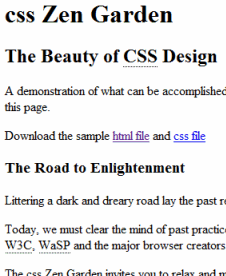
\includegraphics[width=0.3\textwidth]{jeffatwood00.png}\hfill
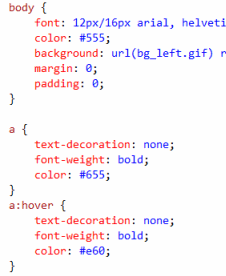
\includegraphics[width=0.3\textwidth]{jeffatwood01.png}\hfill
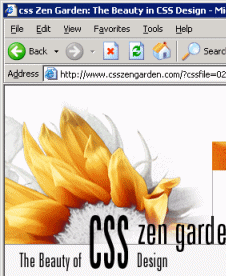
\includegraphics[width=0.3\textwidth]{jeffatwood02.png}

\end{frame}

\sect{HTML, CSS and Browser represent MVC}
\bi
\ii {\bf Model}

The HTML is the "skeleton" of bedrock content. Text that communicates
information to the reader. 

\ii {\bf View}

The CSS adds visual style to the content. It is the "skin" that we use
to flesh out our skeleton and give it a particular look. We can swap
in different skins via CSS without altering the original content in
any way. They are relatively, but not completely, independent. 

\ii{\bf Controller}

The browser is responsible for combining and rendering the CSS and
HTML into a set of final, manipulatible pixels on the screen. It
gathers input from the user and marshals it to any JavaScript code
necessary for the page to function. But here, too, we have
flexibility: we can plug in a different brower and get comparable
results. Some browsers might render it faster, or with more fidelity,
or with more bells and whistles.
\ei
\end{frame}

\sect{Model View Controller (MVC)}
\bi
\ii Data (Model)
\ii An interface to view and modify the data (View)
\ii Operations that can be performed on the data (Controller)
\ei
\end{frame}

\sect{Model View Controller (MVC)}
\bi
\ii
The model represents the data, and does nothing else. The model does
NOT depend on the controller or the view. 
\ii
The view displays the model data, and sends user actions (e.g. button
clicks) to the controller. The view can: 
\bi
\ii
be independent of both the model and the controller; or
\ii
actually be the controller, and therefore depend on the model.
\ei
\ii
The controller provides model data to the view, and interprets user actions such as button clicks. The controller depends on the view and the model. In some cases, the controller and the view are the same object.



\ei
\end{frame}

\sect{The Golden Rule of MVC}

{\LARGE\bf
  The model represents the data, and does nothing else.
  The model does
  NOT depend on the controller or the view.
}

\end{frame}

\sect{Example 1: Address Book}

The model is a list of Person objects, the view is a GUI window that
displays the list of people, and the controller handles actions such
as "Delete person", "Add person", "Email person", etc.

The following
example does {\bf not} use MVC because the model depends on the view.

\begin{Verbatim}[frame=single]
//Example 1:
void Person::setPicture(Picture pict){
    m_picture = pict; //set the member variable
    m_listView->reloadData(); //update the view
}
\end{Verbatim}

\end{frame}

\sect{Example 2: Address Book using MVC}


\begin{Verbatim}[frame=single]
//Example 2:
void Person::setPicture(Picture pict){
    m_picture = pict; //set the member variable
}

void PersonListController::changePictureAtIndex(
      Picture newPict, 
      int personIndex){
  //modify the model
  m_personList[personIndex].setPicture(newPict);
  //update the view
  m_listView->reloadData();
}
\end{Verbatim}
In the above example, the {\tt Person} class knows nothing about the
view. The {\tt PersonListController} handles both changing the model, and
updating the view. The view window tells the controller about user
actions (in this case, it tells the controller that the user changed
the picture of a person).
\end{frame}

\sect{What is the advantage of MVC?}

\bi
\ii  The easiest way to make code overly complex is to put
dependencies everywhere.
\ii Conversely, removing unnecessary dependencies makes delightful
code that is less buggy and easier to maintain because it is {\bf reusable
without modification. } 

\ii The purpose of the controller is to remove the view dependency
from the model. By removing the view dependency from the model, the
model code becomes delightful. 
\ei

\end{frame}

\sect{Continuing our address book example}


The project manager approaches the developer and says:

{\sl
``We love the
contact list window, but we need a second window that displays all the
contacts by their photos only. The photos should be in a table layout,
with five photos per row.''
}

\end{frame}

\sect{Handling the new task with MVC in place}
\bi
\ii
If the application uses MVC, this task is pretty straight
forward. Currently there are three classes: \fbox{\tt Person},
\fbox{\tt PersonListController}, and \fbox{\tt PersonListView}.
\ii
Two classes need to be
created: \fbox{\tt PersonPhotoGridView} and \fbox{\tt
  PersonPhotoGridController}.  The
\fbox{\tt Person} class remains the same, and is easily plugged into the two
different views. How delightful. 
\ei
\end{frame}


\sect{Handling the new task without MVC in place}

\begin{Verbatim}[frame=single]
//Example 3:
void Person::setPicture(Picture pict){
    m_picture = pict; //set the member variable
    //check if it's in a list view
    if(m_listView){ 
      //update the list view
      m_listView->reloadData(); 
    }
    //check if it's in a grid view
    if(m_gridView){ 
      //update the grid view
      m_gridView->reloadData(); 
    }
}
\end{Verbatim}
The model code is starting to turn nasty.

\end{frame}

\sect{More changes and the wonderfulness of MVC }

\bi
\ii
If the project manager then says {\sl ``we're porting the app to a platform
with a different GUI toolkit''} the delightfulness is even more
prominent.
\ii
With MVC, the \fbox{\tt Person} class can be displayed by
different GUI toolkits without any modification. Just make a
controller and a view with the new toolkit, just as you would with the
old toolkit.
\ei


\end{frame}

\sect{More changes without MVC}
{\footnotesize
\begin{Verbatim}[frame=single]
//Example 4:
void Person::setPicture(Picture pict){
    m_picture = pict;
#ifdef ORIGINAL_GUI_TOOLKIT
    if(m_listView){ //check if it's in a list view
        m_listView->reloadData(); //update the list view
    }
    if(m_gridView){ //check if it's in a grid view
        m_gridView->reloadData(); //update the grid view
    }
#endif
#ifdef NEW_GUI_TOOLKIT
    if(m_listView){ //check if it's in a list view
        m_listView->redisplayData(); //update the list view
    }
    if(m_gridView){ //check if it's in a grid view
        m_gridView->redisplayData(); //update the grid view
    }
#endif
}
\end{Verbatim}
}
\end{frame}


\sect{Can we put the controller code in the view?}


One solution to the spaghetti code problem in Example 4 is to move the controller code from the model to the view like so:
{\footnotesize
\begin{Verbatim}[frame=single]
//Example 5:
PersonListView::newPictureClicked(Picture clickedPicture){
    m_selectedPerson.setPicture(clickedPicture);
    this->reloadData();
}
\end{Verbatim}
}
The above example also makes the model reusable, which is the main
advantage of MVC. When the view will only ever display one type of
model object, then combining the view and the controller is fine. For
example, a SinglePersonView will only ever display a Person object, so
the SinglePersonView can double as the controller.


\end{frame}


\sect{MVC can make the view reusable}

However, if the controller is separate from the view then MVC has a
second advantage: \vfill

\centerline{\fbox{\bf MVC can also make the
    view reusable without modification.}}
\vfill

Not only does MVC
make the model delightful, it can also make the view
delightful. Ideally, a list view should be able to display lists of
anything, not just \fbox{\tt Person} objects. The code in Example 5
can not be a generic list view, because it is tied to the model (the
\fbox{\tt Person} class). In the situation where the view should be reusable
(e.g. a list view, or a table view) and the model should be reusable,
MVC is the only thing that will work. The controller removes the
dependencies from both the model and the view, which allows them to be
reused elsewhere.


\end{frame}



\sect{Web sites under MVC}





The model is any of the logic or the database or any of the data
itself. The view is simply how you lay the data out, how it is
displayed. If you want a subset of some data, for example, my opinion
is that is a responsibility of the model. The model knows how to make
a subset. You should not be asking your graphics designer to filter a
list according to age or some other criteria.



\end{frame}

\sect{Web sites under MVC}




The controller in a web app is a bit more complicated, because it has
two parts. The first part is the web server (such as a servlet
container) that maps incoming HTTP URL requests to a particular
handler for that request. The second part is those handlers
themselves, which are in fact often called "controllers." So the C in
a web app MVC includes both the web server "overlord" that routes
requests to handlers and the logic of those handlers themselves, which
pull the data from the database and push it into the template. This
controller also receives HTTP POST requests and processes these,
sometimes updating the database. 
\vfill


I look at a website as nothing but a graph with edges with POSTs and
GETs that routes pages. 
\vfill


\end{frame}

\sect{Virtues of Separating MVC}

My experience is that designers don't understand loops or any kind of
state. They do understand templates with holes in them. Everybody
understands mail merge. And if you say, "Apply the bold template to
this hole," they kind of get that, too. So separating model and view
addresses this very important practical problem of how to have
designers work with coders.
\end{frame}


\sect{Virtues of Separating MVC}
The other problem is there is no way to do multiple site skins
properly if you don't have proper separation of concerns. If you are
doing code generation or sites with different skins on them, there is
no way to properly make a new skin by simply copying and pasting the
old skin and changing it. If you have the view and the logic together,
when you make a copy of the view you copy the logic as well. That
breaks one of our primary rules as developers: have only one place to
change anything. 
\end{frame}
\end{document}
